% Бүлэг 2

\chapter{Шаардлага, зохиомжийн бүлэг} % Бүлгийн нэр
\label{Chapter2} % Энэ бүлэг рүү ишлэл хийх бол \ref{Chapter1} командыг ашигла 

\section{Модулийн үйл ажиллагааны тухай дэлгэрэнгүй }
Энэхүү систем нь Их дээд сургуулийн багш хичээлээ улирлаар үүсгээд, тухайн хичээлийг үзэх оюутнуудыг кодоор нь нэмээд хичээлийн материалаа оруулна.

\section{Модулыг ашиглах хэрэглэгчид}
Их дээд сургуульд суралцдаг оюутан, багш.
\section{Функционал шаардлага}
 Энэхүү модул нь оюутан,багш гэсэн 2 оролцогчтой.
Багш нь: Өөрийн бүртгэлээр нэвтэрч ороод улиралаар хичээлээ үүсгэнэ, хичээлийн материалаа оруулна, тухайн хичээлийг үзэж байгаа оюутнуудыг кодоор нь нэмнэ.
Оюутан: Өөрийн бүртгэлээр нэвтэрч ороод багшийн тавьсан хичээлийн материал, даалгавар, лабораторын удирдамжийг татаж авах буюу систем дээр нээж үзэж болно.

\subsection{Багшын шаардлага}
\begin{itemize}
	
	\item Улирлаар хичээлээ үүсгэх
	\item Хичээлийн материал оруулах хичээлээ сонгох
	\item Хичээлийн материал оруулах
	\item Тухайн хичээлийг үзэж байгаа оюутнуудыг нэмэх
	\item Хайлт хийх
	
	\subsection{Оюутны шаардлага}
	\begin{itemize}
		\item Үүссэн хичээ рүү орох
		\item Хичээлийн материалаа систем дээр нээж харах болон татаж үзэх
	\end{itemize}
	
	\subsection{Системийн шаардлага}
	\begin{itemize}
		\item Тайлан гаргах
		\subitem Хамгийн их файл оруулдаг багш нарын тайланг графикаар харуулах
		\subitem Файлын тоог улирлаар харуулах
		\subitem Татагдсан файлын тоог харуулах
		\item Мэдэгдэл шидэх
	\end{itemize}
\end{itemize}
\section{Функциональ бус шаардлага}
\begin{itemize}
	\item Бүтээгдэхүүний 
	\subitem Хичээлийн материалыг систем дээр харуулах
	\subitem Системийн цагийн хуваарь 24/7 байх
	\subitem Бүх төрлийн төхөөрөмжөөс үзэхэд тохиромжтой хэлбэрээр харагддаг байх буюу загвар нь responsive байх
	
	\item Байгууллагын
	\subitem Өгөгдлийн санд өгөгдлийг нэг форматаар хадгалагддаг байх
	
	\item Гадаад
	\subitem Системд нэвтрэх эрхийг хязгаарлаж, хамгаалдаг байх
	\subitem Бусад албан байгууллагатай хамтран ажилладаг байх
\end{itemize}
\newpage
\section{Юзкейс диаграм}
	\begin{figure}[htbp]
		\centering
		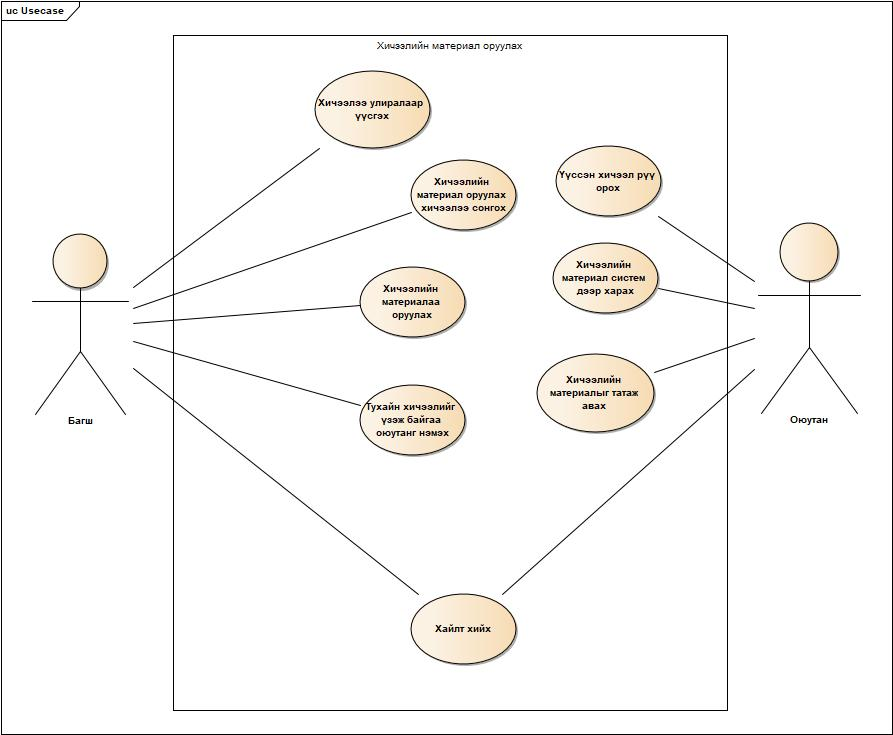
\includegraphics[scale=0.5]{Diagrams/UseCase}
		\caption[Юзкейс диаграм]{Юзкейс диаграм}
		\label{fit:UseCase}
	\end{figure}


\section{Юзкейс диаграмын тодорхойлолт}

\begin{center}
	\begin{table}[!htbp]
		\caption{}
		\begin{tabular}{|p{4cm}|p{11cm}|}
			\hline
			Нэр: & Хичээлийн материал оруулах \\
			\hline
			ID: & 1 \\
			\hline
			Товч тайлбар: & Багш шинээр хичээлээ үүсгэнэ. \\
			\hline
			Триггер: & Багш нь бүртгүүлэх шаардлагатай болсон. \\
			\hline
			Үндсэн оролцогч: & Багш \\
			\hline
			Хоёрдогч оролцогч: & Байхгүй  \\
			\hline
			Өмнөх нөхцөл: &  Веб сервер ажиллагаатай байх\\
			\hline
			Ажлын урсгал: & \begin{enumerate}
				\item Багш хичээлийн материал оруулах сонгосноор энэ юз кейс эхлэнэ. 
				\item Веб сервер нь багшид материал оруулах цонхыг харуулна. 
				\item Багш материалаа оруулна. 
				\item Веб сервер нь багшийн оруулсан мэдээллийг шалгана. 
				\item IF (“мэдээлэл үнэн зөв бол”)
				\begin{enumerate}
					\item[5.1] Веб сервер багшийн оруулсан мэдээллийг баазад хадгална.
					\item[5.2] Веб сервер багшийг амжилттай материал оруулсаныг нь харуулна. 
				\end{enumerate}
				\item ELSE
				\begin{enumerate}
					\item[6.1] Веб сервер нь багшийн оруулсан материалыг шалгана.  
					\item[6.2] Веб сервер нь алдаатай материалыг тодруулж харуулна. 
					\item[6.3] Веб сервер нь материал дахин оруулахыг асууна. 
				\end{enumerate}
			\end{enumerate}
			\\					  \hline
			Дараах нөхцөл: &
			\begin{enumerate}
				\item Багш веб серверд материал оруулсан байна. 
				\item Багшийн оруулсан материал баазад хадгалагдсан байна. 
			\end{enumerate}	   
			\\				   \hline
			Альтернатив урсгал: &  \begin{enumerate}
				\item Багш материалыг цуцалсан.
				\item Веб сервер дээр алдаа гарсан. 
			\end{enumerate}
			\\	\hline
		\end{tabular}
	\end{table}
\end{center}

\begin{center}
	\begin{table}[!htbp]
		\caption{}
		\begin{tabular}{|p{4cm}|p{11cm}|}
			\hline
			Нэр: & Хичээлээ улирлаар үүсгэх\\
			\hline
			ID: & 1 \\
			\hline
			Товч тайлбар: & Багш шинээр улирлаа үүсгэнэ. \\
			\hline
			Триггер: & Багш улирал үүсгэх шаардлагатай болсон. \\
			\hline
			Үндсэн оролцогч: & Багш \\
			\hline
			Хоёрдогч оролцогч: & Байхгүй  \\
			\hline
			Өмнөх нөхцөл: &  Веб сервер ажиллагаатай байх\\
			\hline
			Ажлын урсгал: & \begin{enumerate}
				\item Багш улиралаар хичээлээ үүсгэхийг сонгосоноор энэ юз кейс эхлэнэ. 
				\item Веб сервер нь багшид хичээл улиралаар үүсгэх цонхыг харуулна. 
				\item Багш нь улирал болон хичээлийн мэдээллийг оруулна. 
				\item Веб сервер нь багшийн оруулсан мэдээллийг шалгана. 
				\item IF (“мэдээлэл үнэн зөв бол”)
				\begin{enumerate}
					\item[5.1] Веб сервер багшийн оруулсан мэдээллийг баазад хадгална.
					\item[5.2] Веб сервер багшийг хичээллээ улирлаар амжилттай үүсгэсэнийг нь харуулна. 
				\end{enumerate}
				\item ELSE
				\begin{enumerate}
					\item[6.1] Веб сервер нь багшийн оруулсан мэдээлэл бүрийг шалгана.  
					\item[6.2] Веб сервер нь алдаатай оруулсан мэдээллийг тодруулж харуулна. 
					\item[6.3] Веб сервер нь мэдээллийг дахин оруулахыг асууна. 
				\end{enumerate}
			\end{enumerate}
			\\					  \hline
			Дараах нөхцөл: &
			\begin{enumerate}
				\item Багш веб серверд улиралаа хичээлээ үүсгэсэн байна. 
				\item Багшийн оруулсан мэдээлэл баазад хадгалагдсан байна. 
			\end{enumerate}	   
			\\				   \hline
			Альтернатив урсгал: &  \begin{enumerate}
				\item Багш улиралыг цуцалсан.
				\item Веб сервер дээр алдаа гарсан. 
			\end{enumerate}
			\\	\hline
		\end{tabular}
	\end{table}
\end{center}

\begin{center}
	\begin{table}[!htbp]
		\caption{} 
		\begin{tabular}{|p{4cm}|p{11cm}|}
			\hline
			Нэр: & Хайлт хийх  \\
			\hline
			ID: & 7 \\
			\hline
			Товч тайлбар: & Оюутан, Багш вебээс өөрийн хүссэн мэдээллийг хайна.  \\
			\hline
			Үндсэн оролцогч: & Оюутан, Багш \\
			\hline
			Хоёрдогч оролцогч: & Байхгүй  \\
			\hline
			Өмнөх нөхцөл: &  Вебд нэвтэрсэн байх \\
			\hline
			Ажлын урсгал: & \begin{enumerate}
				\item Оюутан, Багш хайлт хийх хэсгийг сонгосоноор энэхүү юзкейс эхэлнэ
				\item Оюутан, Багш хайлтын утгаа оруулна
				\item IF(Хайлтын утга алдаатай бол)
				\begin{enumerate}
					\item[6.1] Веб хайлтын утга алдаатайг оюутан, багшид мэдэгдэнэ.
					\item[6.2] Веб оюутан, багшид зөв хайлтын жишээ утга харуулна
				\end{enumerate}	
				\item ELSE IF(Таны хайсан утга )
				\begin{enumerate}
					\item[7.1] Веб таны хайсан утга илэрцгүй 
				\end{enumerate}
				\item Вэб хайлтанд илэрсэн утгуудыг харуулна
			\end{enumerate} 	\\
			\hline
			Дараах нөхцөл: & Оюутан, багш вебээс хүссэн хайлтаа олсон байна. \\
			\hline
			Альтернатив урсгал: & Оюутан, багшийн хайлт илэрцгүй байна.\\
			\hline
		\end{tabular}
	\end{table}
\end{center}

%-------------------------------------------------------------------------------
\newpage
\section{ERD диаграм}

\begin{figure}[!h]
	\centering
	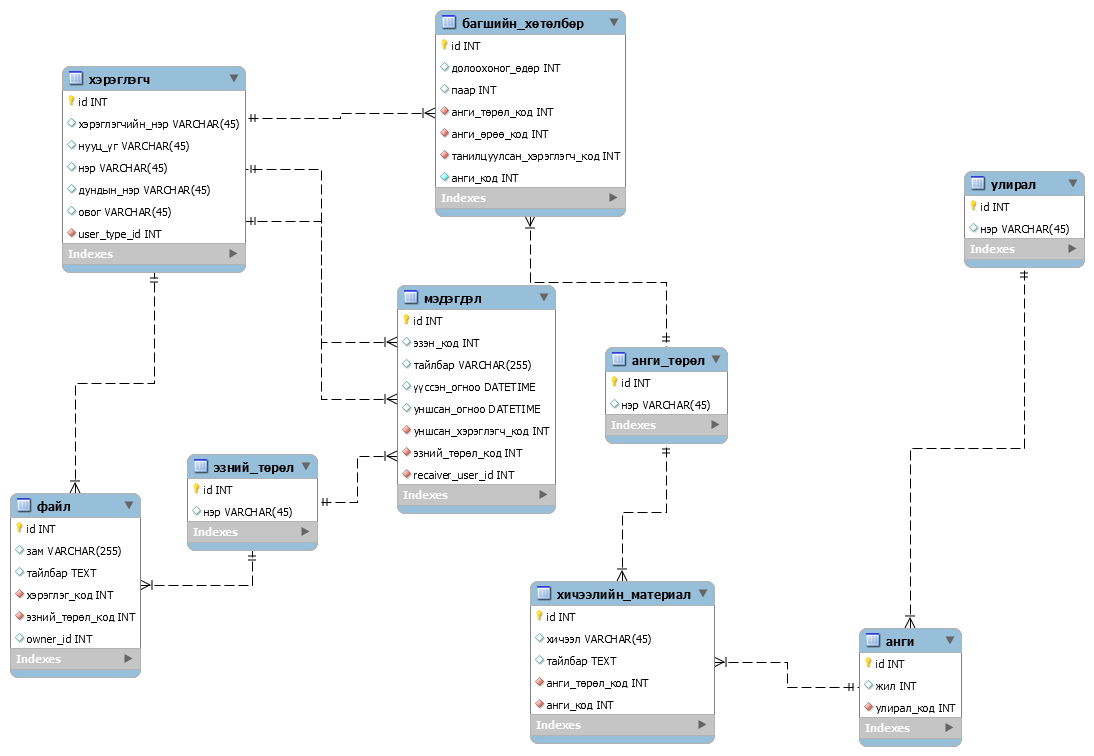
\includegraphics[scale=0.3]{Diagrams/S}
	\caption[ERD диаграм]{ERD диаграм}
	\label{fig:SClass}
\end{figure}

%--------------------------------------------------------------


\section{Үйл ажиллагааны диаграм}

\begin{figure}
	\centering
	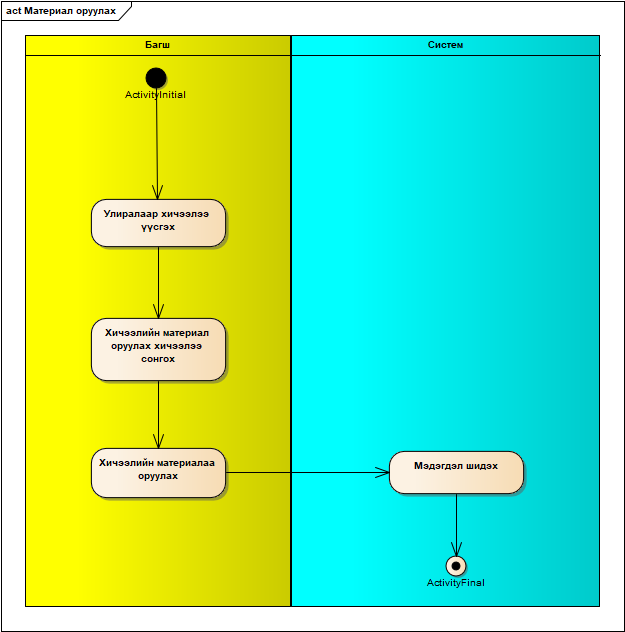
\includegraphics[angle=90, scale=0.7]{Diagrams/activity}
	\caption[Багш хичээлийн материал оруулах үйл ажиллагааны диаграм]{Багш хичээлийн материал оруулах үйл ажиллагааны диаграмм}
	\label{text}
\end{figure}
\newpage
\begin{figure}
	
	\centering
	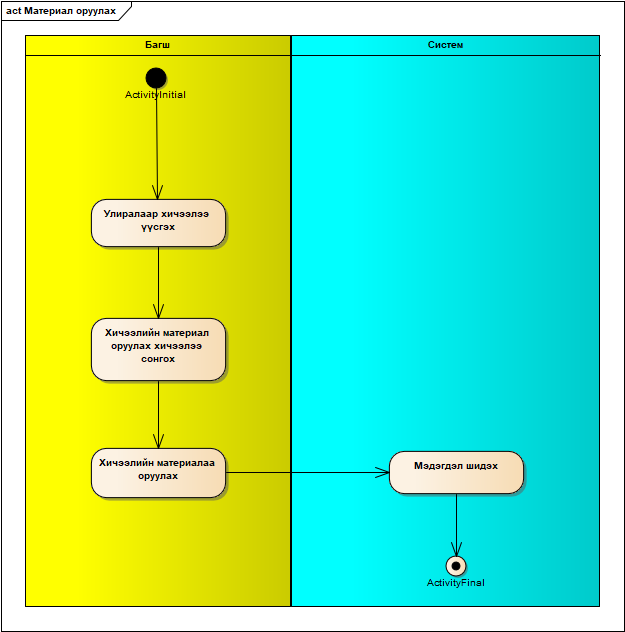
\includegraphics[angle=90, scale=0.75]{Diagrams/activity1}
	\caption[Багш тухайн хичээлийг үзэж байгаа оюутанг нэмэх үйл ажиллагааны диаграм]{Багш тухайн хичээлийг үзэж байгаа оюутанг нэмэх үйл ажиллагааны диаграм}
	\label{text}
\end{figure}

\newpage
\begin{figure}
	\centering
	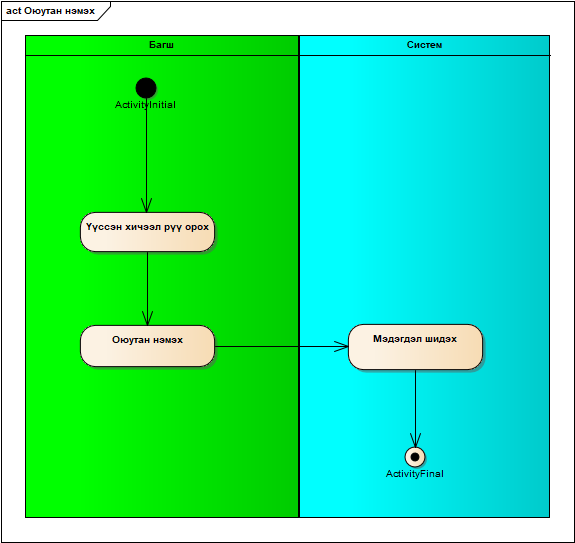
\includegraphics[angle=90, scale=0.8]{Diagrams/activity3}
	\caption[Оюутан хичээлийн материал татаж авах үйл ажиллагааны диаграм]{Оюутан хичээлийн материал татаж авах үйл ажиллагааны диаграм}
	\label{text}
\end{figure}

\newpage
\section{Дарааллын диаграм}
\newpage
\begin{figure}
	\centering
	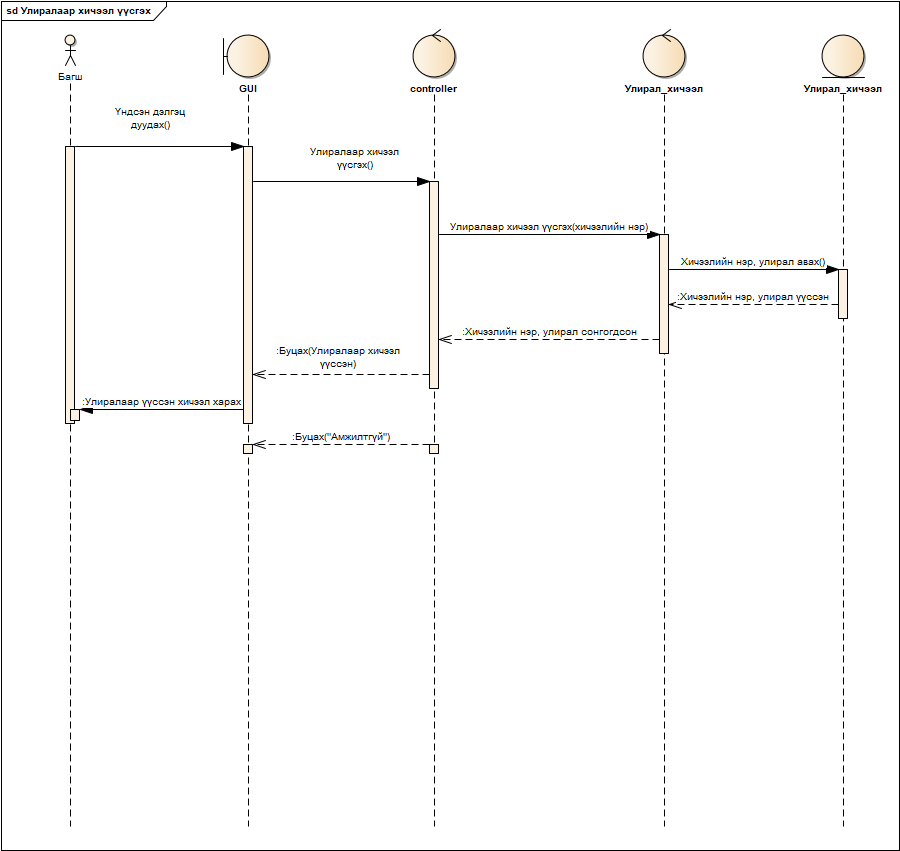
\includegraphics[angle=90, scale=0.5]{Diagrams/Sequence1}
	\caption[Багш улиралаар хичээл үүсгэх үйлдлийн дарааллын диаграм]{Багш улиралаар хичээл үүсгэх үйлдлийн дарааллын диаграм}
	\label{text}
\end{figure}

\newpage
\begin{figure}
	\centering
	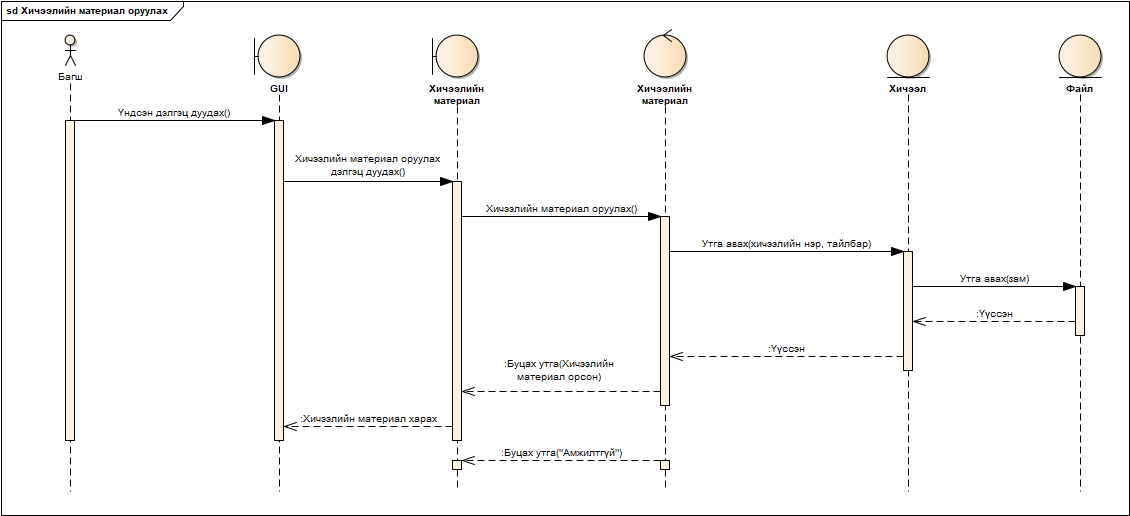
\includegraphics[angle=90, scale=0.5]{Diagrams/Sequence2}
	\caption[Багш хичээлийн материал оруулах үйлдлийн дарааллын диаграм]{Багш хичээлийн материал оруулах үйлдлийн дарааллын диаграм}
	\label{text}
\end{figure}

\newpage
\begin{figure}
	\centering
	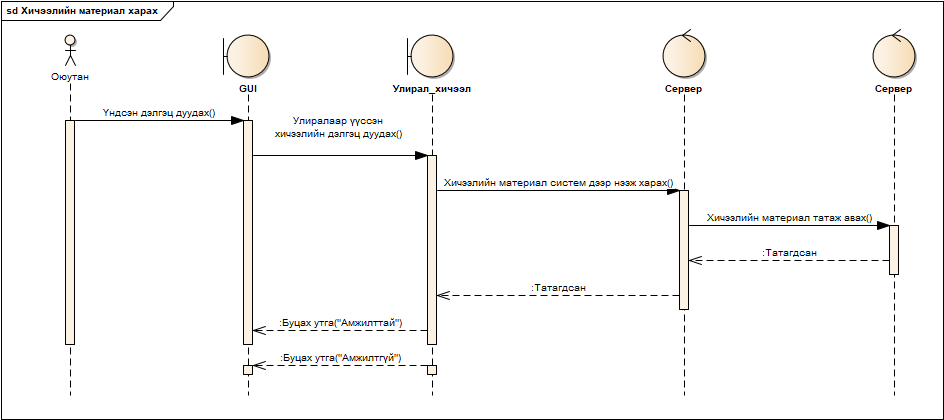
\includegraphics[angle=90, scale=0.5]{Diagrams/Sequence3}
	\caption[Оюутан хичээлийн материал татаж авах үйлдлийн дарааллын диаграм]{Оюутан хичээлийн материал татаж авах үйлдлийн дарааллын диаграм}
	\label{text}
\end{figure}

\newpage
\section{Класс диаграм}
\begin{figure}
	\centering
	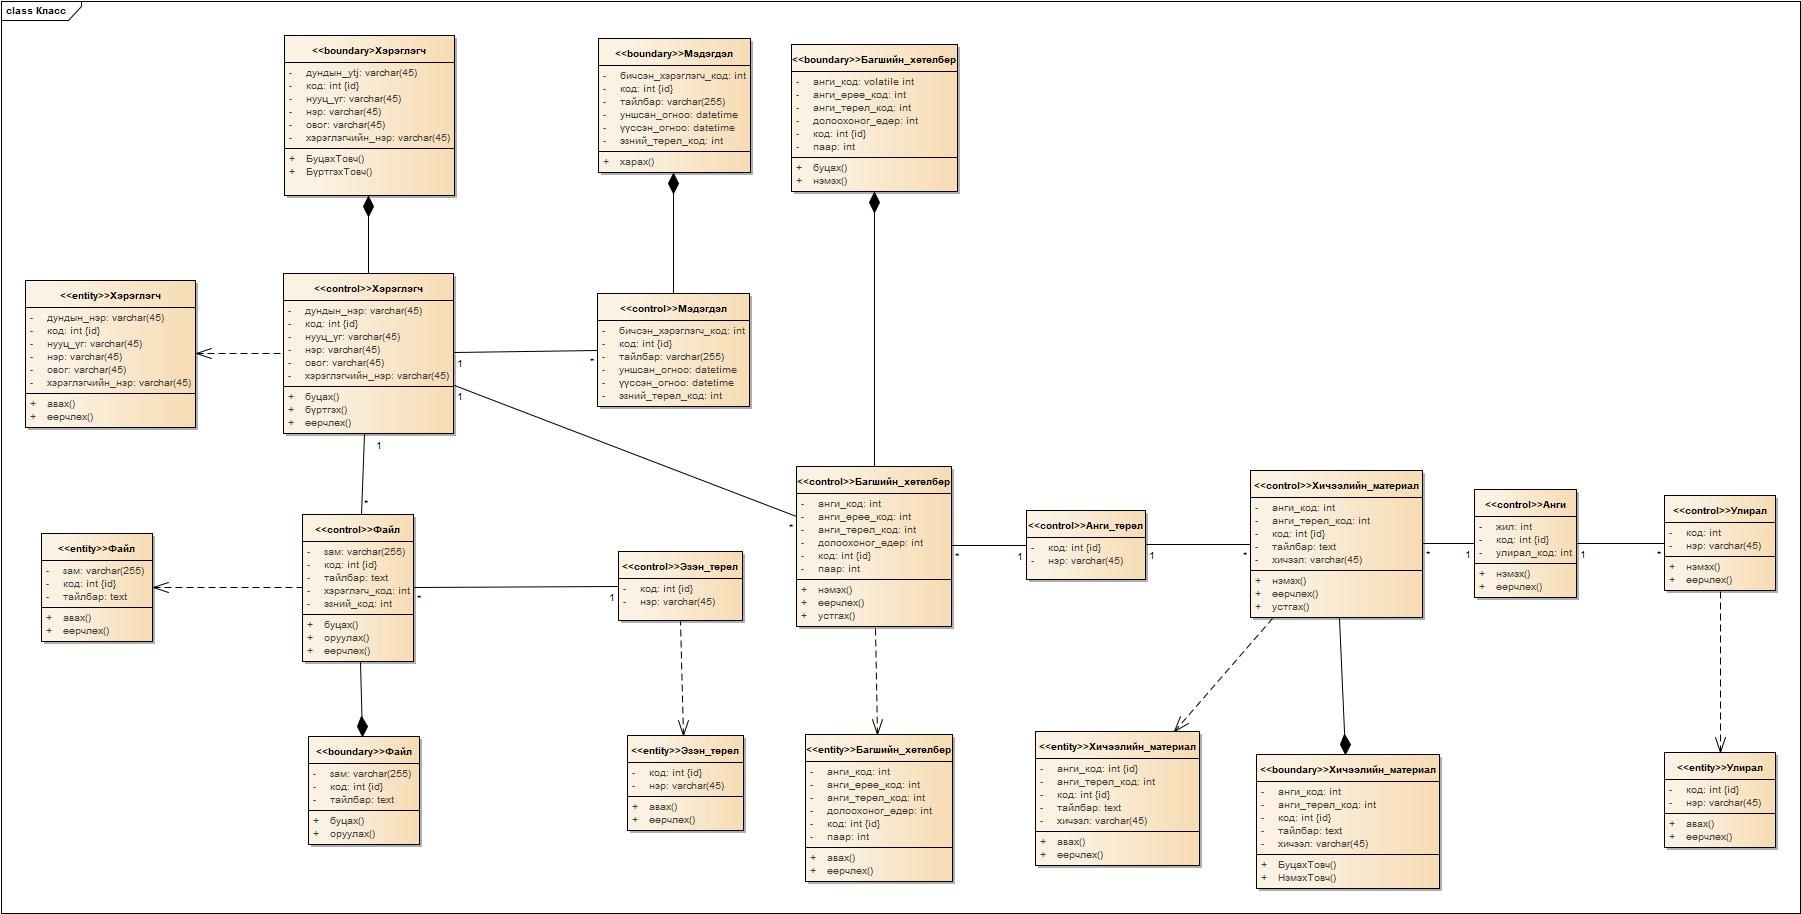
\includegraphics[angle=90, scale=0.4]{Diagrams/SClass}
	\caption[Класс диаграм]{Класс диаграм}
	\label{text}
\end{figure}

\newpage
\section{Бүлгийн дүгнэлт}
Хэрэглэгчийн шаардлагаа тодорхойлж тодорхойлсон шаардлага бүрээ нягтлан хянаж функционал болон фунционал бусаар нь ялгасан. Функционал шаардлага дээрээ үндэслэн юз кейс диаграмаа гаргасан ба бүх  юзкейс бүрт тодорхойлолт гаргасан. Мөн үйл ажиллагааны диаграм зурсан үйл ажиллагааг нь илүү нарийн ойлгомжтой болгож өгч байна.

